\documentclass[xcolor=pdftex,dvipsnames,table]{beamer}
\mode<presentation>
\usetheme{boxes}
\setbeamertemplate{navigation symbols}{}
% http://www.latex-community.org/forum/viewtopic.php?f=4&t=6694
\setbeamertemplate{navigation symbols}{\raisebox{5pt}{\makebox[\paperwidth]{\hfill\makebox[10pt]{\scriptsize\insertframenumber\vspace{1ex}}}}}
\setbeamertemplate{footline}[frame number]
\setbeamertemplate{blocks}[shadow=false]
\setbeamercolor*{block title}{fg=structure,bg=RoyalBlue!10}
\setbeamercolor*{block title example}{fg=BrickRed,bg=Goldenrod!10}
\setbeamercolor*{block title alerted}{fg=white,bg=black}
\addtobeamertemplate{block begin}{\pgfsetfillopacity{0.8}}{\pgfsetfillopacity{1}}
\rowcolors{1}{RoyalBlue!20}{RoyalBlue!5}

%\DeclareGraphicsRule{*}{mps}{*}{}

\usepackage{latexsym}
\usepackage{hyperref}

\raggedright

\newcount\lecturecount
\lecturecount=0
\AtBeginLecture{%
    \advance\lecturecount by 1
    \date{}
    \begin{frame}
    \begin{center}
    \titlepage
    \ifnum\lecturecount=1
    Part \the\lecturecount: \insertlecture
    \else
    Part \the\lecturecount: \insertlecture
    \fi
    \end{center}
    \end{frame}
}

\usepackage{CJKutf8}
\begin{document}

\title{\color{blue}Natural Language Processing}

\author{Anoop Sarkar \\ {\tt http://anoopsarkar.github.io/nlp-class}}
\institute{}
%\date{}
     
{
\setbeamertemplate{navigation symbols}{}
\addtocounter{framenumber}{-1}
\begin{frame}
\begin{center}
\vspace{1cm}
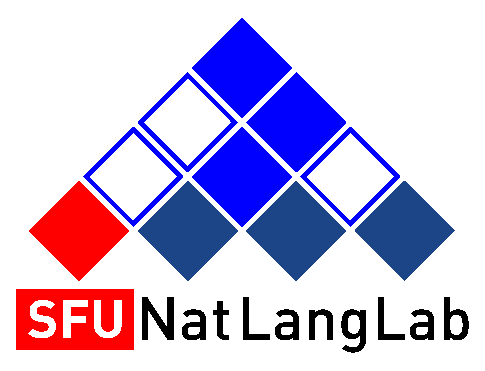
\includegraphics[scale=0.4]{figures/natlang-cky-logo.eps}
\end{center}
\titlepage
\end{frame}
}



\lecture{Introducing Hidden Markov Models}{}
\section{Introducing HMMs}

\begin{frame}
\frametitle{Modelling pairs of sequences}
\begin{block}{Input: sequence of words; Output: sequence of labels}
\begin{tabular}{lllllll}
\textbf{Input} & British & left & waffles & on & Falkland & Islands \pause \\
\textbf{Output1} & N & N & V & P & N & N \\
\textbf{Output2} & N & V & N & P & N & N \\
$\vdots$ & & & & & & 
\end{tabular}

\begin{description}
\item[N] Noun, e.g.\ islands
\item[V] Verb, e.g.\ leave, left
\item[P] Preposition, e.g.\ on
\end{description}
\end{block}
\end{frame}

\begin{frame}
\frametitle{Modelling pairs of sequences}
\begin{block}{Input: sequence of words; Output: sequence of labels}
\begin{tabular}{lllllll}
\textbf{Input} & British & left & waffles & on & Falkland & Islands \pause \\
\textbf{Output1} & N & N & V & P & N & N \\
\textbf{Output2} & N & V & N & P & N & N \\
$\vdots$ & & & & & & 
\end{tabular}
\end{block}

\pause
\begin{block}{}
\begin{itemize}
\item 3 states: ${\cal S} = \{ N, V, P \}$
\item Input sequence: $x_1, x_2, \ldots, x_n$
\item Output sequence: $t_1, t_2, \ldots, t_n$ where $t_i \in {\cal S}$
\item \callouts{blue}{$\mid {\cal S} \mid^n$}{How many output sequences?}
\end{itemize}
\end{block}
\end{frame}

\begin{frame}
\frametitle{Modelling pairs of sequences}
\begin{block}{Input: sequence of characters; Output: sequence of labels}
\begin{tabular}{lll}
\textbf{Input} & 
\begin{CJK*}{UTF8}{gbsn}
北京大学生比赛
\end{CJK*} & 7 chars \pause \\
\textbf{Output1} & 
BIBIIBI & 7 labels \\
\textbf{Output2} & 
BIIIBBI & 7 labels \\ 
$\vdots$ & & 7 labels 
\end{tabular}
\begin{description}
\item[B] Begin word
\item[I] Inside word
\end{description}
\pause 
\begin{description}
\item[BIBIIBI] 
\begin{CJK*}{UTF8}{gbsn}
北京---大学生---比赛
\end{CJK*}
(Beijing student competition)
\item[BIIIBBI] 
\begin{CJK*}{UTF8}{gbsn}
北京大学---生---比赛 
\end{CJK*}
(Peking University Health Competition)
\end{description}
\end{block}
\end{frame}

\section{Constructing a HMM model}
\begin{frame}
\frametitle{Hidden Markov Models}
\begin{block}{}
\begin{itemize}[<+->]
\item Input: $x$
\item Output space: ${\cal Y}(x)$
\item Output: $y \in {\cal Y}(x)$
\item We want to learn a function $f$ such that $f(x) = y$
\end{itemize}
\end{block}
\end{frame}

\begin{frame}
\frametitle{Hidden Markov Models}
\begin{block}{Conditional model}
\begin{itemize}[<+->]
\item Construct function $f$ using a conditional probability:
\[ f(x) = \arg\max_{y \in {\cal Y}(x)} p(y \mid x) \]
\item We can construct this function $f$ using two principles:
\begin{itemize}
\item Discriminative learning: find the best output $y$ given input $x$
\item Generative modelling: model the joint probability $p(x,y)$ to find $p(y \mid x)$
\end{itemize}
\end{itemize}
\end{block}
\end{frame}

\begin{frame}
\frametitle{Hidden Markov Models}
\begin{block}{Generative Model}
\begin{itemize}[<+->]
\item Start from the joint probability $p(x,y)$:
\[ p(x,y) = p(y) p(x \mid y) \]
\item Also:
\[ p(x,y) = p(x) p(y \mid x) \]
\end{itemize}
\end{block}
\pause
\begin{block}{Bayes Rule:}
\[ p(y \mid x) = \frac{ p(y) p(x \mid y) }{ p(x) } \]
\end{block}
\end{frame}

\begin{frame}
\frametitle{Hidden Markov Models}
\begin{block}{Generative Model}
\begin{itemize}[<+->]
\item Bayes Rule:
\[ p(y \mid x) = \frac{ p(y) p(x \mid y) }{ p(x) } \]
\item where:
\[ p(x) = \sum_{y \in {\cal Y}(x)} p(x, y) = \sum_{y \in {\cal Y}(x)} p(y) p(x \mid y) \]
\item So using a generative model, we can find the best output $y$ using:
\[ p(y \mid x) = \frac{ p(y) p(x \mid y) }{ \sum_{y \in {\cal Y}(x)} p(y) p(x \mid y) } \]
\end{itemize}
\end{block}
\end{frame}

\lecture{Algorithms for Hidden Markov Models}{}
\section{Algorithms for HMMs}

\begin{frame}
\frametitle{Hidden Markov Model}
\[
\textrm{Model $\theta$} = \left\{ 
\begin{array}{ll} 
\pi_i & \textrm{$p(i)$: starting at state $i$} \\ 
a_{i,j} & \textrm{$p(j \mid i)$: transition to state $i$ from state $j$} \\ 
b_i(o) & \textrm{$p( o \mid i)$: output $o$ at state $i$}
\end{array} 
\right.\]

\begin{center}
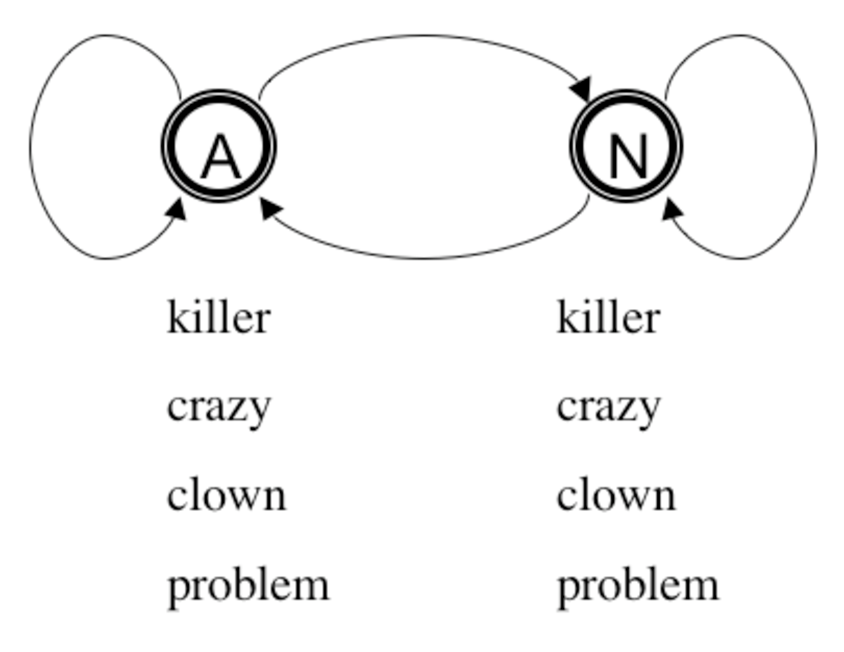
\includegraphics[scale=.4]{figures/hmmfig}
\end{center}
\end{frame}

\begin{frame}
\frametitle{Hidden Markov Model Algorithms}
\begin{itemize}
\item HMM as parser: compute the best sequence of states for a given observation sequence.
\item HMM as language model: compute probability of given observation sequence.
\item HMM as learner: given a corpus of observation sequences, learn its distribution, i.e. learn the parameters of the HMM from the corpus.
\begin{itemize}
\item Learning from a set of observations with the sequence of states provided (states are not hidden) {\color{blue} [Supervised Learning]}
\item Learning from a set of observations without any state information. {\color{blue} [Unsupervised Learning]}
\end{itemize}
\end{itemize}
\end{frame}

\section{HMM as Parser}

\begin{frame}
\frametitle{HMM as Parser}
\begin{center}
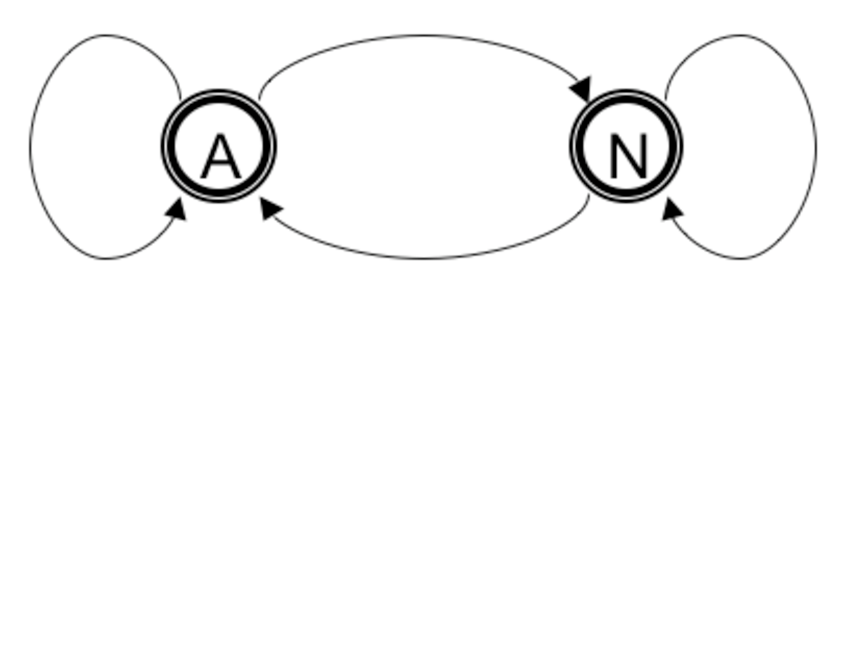
\includegraphics[scale=.25]{figures/hmmfig2}
\end{center}
{\color{blue}
\begin{center}
\begin{columns}[c]
\column{0.5in}
\[ \pi = \begin{array}{|l|l|}
\hline
A & 0.25 \\ \hline
N & 0.75 \\ \hline
\end{array}
\]
\pause
\column{0.65in}
\[ a = \begin{array}{|l|l|l|}
\hline
a_{i,j} & A & N \\ \hline
A & 0.0 & 1.0 \\ \hline
N & 0.5 & 0.5 \\ \hline
\end{array}
\]
\end{columns}
\pause
\begin{columns}[c]
\column{3in}
\[ b = \begin{array}{|l|l|l|l|l|}
\hline
b_i(o) & clown & killer & problem & crazy \\ \hline
A & 0 & 0 & 0 & 1 \\ \hline
N & 0.4 & 0.3 & 0.3 & 0 \\ \hline
\end{array}
\]
\end{columns}
\end{center}
}
\pause
\begin{quote}
The task: for a given observation sequence find the most likely state sequence.
$a_{i,j} = p(j \mid i)$ and $b_i(o) = p(o \mid i)$
\end{quote}
\end{frame}

\begin{frame}
\frametitle{HMM as Parser}
\begin{center}
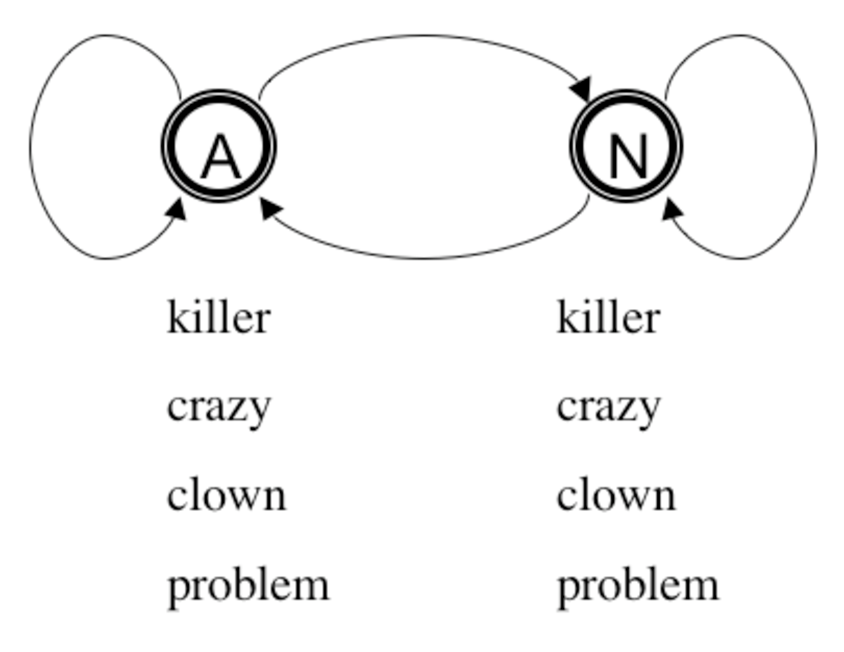
\includegraphics[scale=.3]{figures/hmmfig}
\end{center}
\begin{itemize}[<+->]
\item Find most likely sequence of states for {\it killer clown}
\item Score every possible sequence of states: AA, AN, NN, NA
\begin{itemize}[<+->]
\item {\color{blue} P(killer clown, AA) = $\pi_A \cdot b_A(\textit{killer}) \cdot a_{A,A} \cdot b_A(\textit{clown})$ = $0.0$}
\item {\color{blue} P(killer clown, AN) = $\pi_A \cdot b_A(\textit{killer}) \cdot a_{A,N} \cdot b_N(\textit{clown})$ = $0.0$}
\item {\color{blue} P(killer clown, NN) = $\pi_N \cdot b_N(\textit{killer}) \cdot a_{N,N} \cdot b_N(\textit{clown})$ = $0.75 \cdot 0.3 \cdot 0.5 \cdot 0.4$ = $0.045$}
\item {\color{blue} P(killer clown, NA) = $\pi_N \cdot b_N(\textit{killer}) \cdot a_{N,A} \cdot b_A(\textit{clown})$ = $0.0$}
\end{itemize}
\item Pick the state sequence with highest probability (NN=$0.045$).
\end{itemize}
\end{frame}

\begin{frame}
\frametitle{HMM as Parser}
\begin{itemize}[<+->]
\item As we have seen, for input of length 2, and a HMM with 2 states there are $2^2$ possible state sequences.
\item In general, if we have $q$ states and input of length $T$ there are $q^T$ possible state sequences.
\item Using our example HMM, for input {\it killer crazy clown problem} we will have $2^4$ possible state sequences to score.
\item Our naive algorithm takes exponential time to find the best state sequence for a given input.
\item The {\bf Viterbi algorithm} uses dynamic programming to provide the best state sequence with a time complexity of $q^2 \cdot T$
\end{itemize}
\end{frame}

\lecture{Viterbi Algorithm for HMMs}{}
\section{Viterbi Algorithm for HMMs}

\begin{frame}
\frametitle{Viterbi Algorithm for HMMs}
\begin{itemize}[<+->]
\item For input of length $T$: $o_1, \ldots, o_T$, we want to find the sequence of states $s_1, \ldots, s_T$
\item Each $s_t$ in this sequence is one of the states in the HMM.
\item So the task is to find the most likely sequence of states:
\[ \arg\max_{s_1, \ldots, s_T} P(o_1, \ldots, o_T, s_1, \ldots, s_T) \]
\item The Viterbi algorithm solves this by creating a table $V[s,t]$ where $s$ is one of the states, and $t$ is an index between $1, \ldots, T$.
\end{itemize}
\end{frame}

\begin{frame}
\frametitle{Viterbi Algorithm for HMMs}
\begin{center}
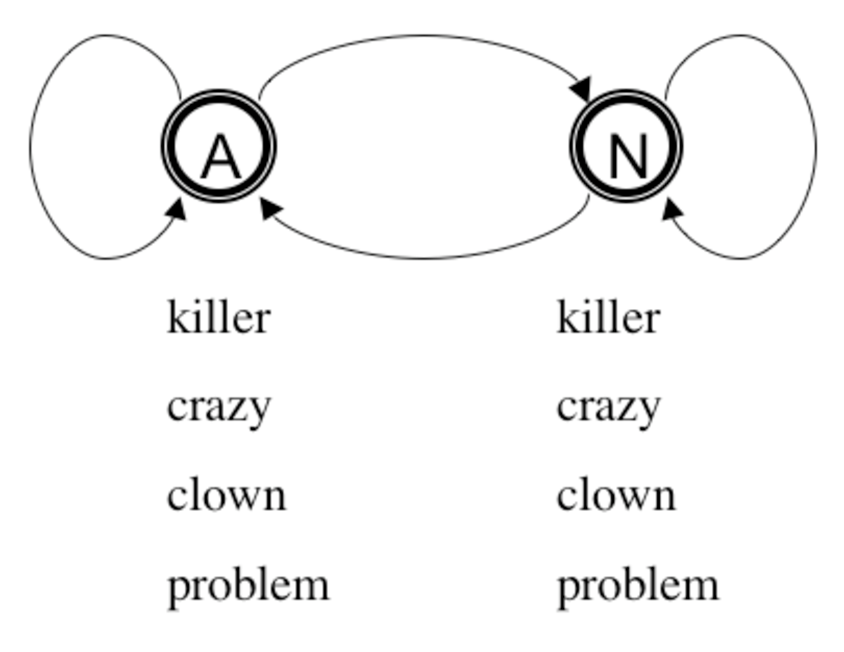
\includegraphics[scale=.3]{figures/hmmfig}
\end{center}
\begin{itemize}[<+->]
\item Consider the input {\it killer crazy clown problem}
\item So the task is to find the most likely sequence of states:
\[ \arg\max_{s_1, s_2, s_3, s_4} P(\textit{killer crazy clown problem}, s_1, s_2, s_3, s_4) \]
\item A sub-problem is to find the most likely sequence of states for {\it killer crazy clown}:
\[ \arg\max_{s_1, s_2, s_3} P(\textit{killer crazy clown}, s_1, s_2, s_3) \]
\end{itemize}
\end{frame}

\begin{frame}
\frametitle{Viterbi Algorithm for HMMs}
\begin{itemize}[<+->]
\item In our example there are two possible values for $s_4$:
\begin{eqnarray*}
\lefteqn{\max_{s_1, \ldots, s_4} P(\textit{killer crazy clown problem}, s_1, s_2, s_3, s_4) =} \\
&& \max \left\{ {\color{blue} \max_{s_1, s_2, s_3} P(\textit{killer crazy clown problem}, s_1, s_2, s_3, N) }, \right. \\
&&  \left. {\color{blue} \max_{s_1, s_2, s_3} P(\textit{killer crazy clown problem}, s_1, s_2, s_3, A) } \right\}
\end{eqnarray*}
\item Similarly:
\begin{eqnarray*}
\lefteqn{\max_{s_1, \ldots, s_3} P(\textit{killer crazy clown}, s_1, s_2, s_3) =} \\
&& \max \left\{ {\color{blue} \max_{s_1, s_2} P(\textit{killer crazy clown}, s_1, s_2, N) }, \right. \\
&&  \left. {\color{blue} \max_{s_1, s_2} P(\textit{killer crazy clown}, s_1, s_2, A) } \right\}
\end{eqnarray*}
\end{itemize}
\end{frame}

\begin{frame}
\frametitle{Viterbi Algorithm for HMMs}
\begin{itemize}[<+->]
\item Putting them together:
\begin{eqnarray*}
\lefteqn{P(\textit{killer crazy clown problem}, s_1, s_2, s_3, N) =} \\
&& \max \left\{ P(\textit{killer crazy clown}, s_1, s_2, N) \cdot a_{N,N} \cdot b_N(\textit{problem}), \right. \\
&&  \left. P(\textit{killer crazy clown}, s_1, s_2, A) \cdot a_{A,N} \cdot b_N(\textit{problem}) \right\}
\end{eqnarray*}
\begin{eqnarray*}
\lefteqn{P(\textit{killer crazy clown problem}, s_1, s_2, s_3, A) =} \\
&& \max \left\{ P(\textit{killer crazy clown}, s_1, s_2, N) \cdot a_{N,A} \cdot b_A(\textit{problem}), \right. \\
&&  \left. P(\textit{killer crazy clown}, s_1, s_2, A) \cdot a_{A,A} \cdot b_A(\textit{problem}) \right\}
\end{eqnarray*}
\item The best score is given by:
\begin{eqnarray*}
\lefteqn{\max_{s_1, \ldots, s_4} P(\textit{killer crazy clown problem}, s_1, s_2, s_3, s_4) =} \\
&& \max_{N,A} \left\{ {\color{blue}  \max_{s_1, s_2, s_3} P(\textit{killer crazy clown problem}, s_1, s_2, s_3, N),  } \right. \\
&&  \left. {\color{blue}  \max_{s_1, s_2, s_3} P(\textit{killer crazy clown problem}, s_1, s_2, s_3, A) } \right\} 
\end{eqnarray*}
\end{itemize}
\end{frame}

\begin{frame}
\frametitle{Viterbi Algorithm for HMMs}
\begin{itemize}[<+->]
\item Provide an index for each input symbol:\\
 {\it 1:killer 2:crazy 3:clown 4:problem} 
\begin{eqnarray*}
V[N, 3] &=& \max_{s_1, s_2} P(\textit{killer crazy clown}, s_1, s_2, N) \\
V[N, 4] &=& \max_{s_1, s_2, s_3} P(\textit{killer crazy clown problem}, s_1, s_2, s_3, N)
\end{eqnarray*}

\item Putting them together:
\begin{eqnarray*}
V[N,4] &=& \max \left\{ {\color{blue} V[N,3] \cdot a_{N,N} \cdot b_N(\textit{problem}) }, \right.\\
&& \left. {\color{blue} V[A,3] \cdot a_{A,N} \cdot b_N(\textit{problem}) } \right\}
\end{eqnarray*}
\begin{eqnarray*}
V[A,4] &=& \max \left\{ {\color{blue} V[N,3] \cdot a_{N,A} \cdot b_A(\textit{problem}) }, \right.\\
&& \left. {\color{blue} V[A,3] \cdot a_{A,A} \cdot b_A(\textit{problem}) } \right\}
\end{eqnarray*}
\item The best score for the input is given by:
\( \max \left\{ V[N,4] , V[A,4] \right\} \)
\item To extract the best sequence of states we backtrack (same trick as obtaining alignments from minimum edit distance)
\end{itemize}
\end{frame}

\begin{frame}
\frametitle{Viterbi Algorithm for HMMs}
\begin{itemize}[<+->]
\item For input of length $T$: $o_1, \ldots, o_T$, we want to find the sequence of states $s_1, \ldots, s_T$
\item Each $s_t$ in this sequence is one of the states in the HMM.
\item For each state $q$ we initialize our table: $V[q,1] = \pi_q \cdot b_q(o_1)$ 
\item Then compute for $t = 1 \ldots T-1$ for each state $q$:
\[ V[q, t+1] = \max_{q'} \left\{ V[q', t] \cdot a_{q',q} \cdot b_q(o_{t+1}) \right\} \]
\item After the loop terminates, the best score is $\max_q V[q,T]$
\end{itemize}
\end{frame}

\begin{frame}[fragile]
\frametitle{Learning from Fully Observed Data}
{\color{blue}
\begin{center}
\begin{columns}[c]
\column{0.5in}
\[ \pi = \begin{array}{|l|l|}
\hline
A & 0.25 \\ \hline
N & 0.75 \\ \hline
\end{array}
\]
\pause
\column{0.65in}
\[ a = \begin{array}{|l|l|l|}
\hline
a_{i,j} & A & N \\ \hline
A & 0.0 & 1.0 \\ \hline
N & 0.5 & 0.5 \\ \hline
\end{array}
\]
\end{columns}
\pause
\begin{columns}[c]
\column{3in}
\[ b = \begin{array}{|l|l|l|l|l|}
\hline
b_i(o) & clown & killer & problem & crazy \\ \hline
A & 0 & 0 & 0 & 1 \\ \hline
N & 0.4 & 0.3 & 0.3 & 0 \\ \hline
\end{array}
\]
\end{columns}
\end{center}
\pause
\smallskip
Viterbi algorithm:\\
\begin{center}
\begin{tabular}{|p{1cm}|p{2cm}|p{2cm}|p{2cm}|p{2cm}|}
\hline
{\bf V} & killer:1 & crazy:2 & clown:3 & problem:4 \\ \hline
A & & & & \\ \hline
N & & & & \\ \hline
\end{tabular}
\end{center}
}
\end{frame}

\setbeamercovered{again covered={\opaqueness<1->{25}}}
\begin{frame}[fragile]
\frametitle{Learning from Fully Observed Data}
{\color{blue}
\begin{center}
\begin{columns}[c]
\column{0.5in}
\[ \pi = \begin{array}{|l|l|}
\hline
A & 0.25 \\ \hline
N & 0.75 \\ \hline
\end{array}
\]
\column{0.65in}
\[ a = \begin{array}{|l|l|l|}
\hline
a_{i,j} & A & N \\ \hline
A & 0.0 & 1.0 \\ \hline
N & 0.5 & 0.5 \\ \hline
\end{array}
\]
\end{columns}
\begin{columns}[c]
\column{3in}
\[ b = \begin{array}{|l|l|l|l|l|}
\hline
b_i(o) & clown & killer & problem & crazy \\ \hline
A & 0 & 0 & 0 & 1 \\ \hline
N & 0.4 & 0.3 & 0.3 & 0 \\ \hline
\end{array}
\]
\end{columns}
\end{center}
\smallskip
Viterbi algorithm:\\
\begin{center}
\begin{tabular}{|p{1cm}|p{2cm}|p{2cm}|p{2cm}|p{2cm}|}
\hline
{\bf V} & killer:1 & crazy:2 & clown:3 & problem:4 \\ \hline
A & \hspace{0pt}\uncover<2>{0} & \hspace{0pt}\uncover<4>{0.1125} & \hspace{0pt}\uncover<6>{0} & \hspace{0pt}\uncover<8>{0} \\ \hline
N & \hspace{0pt}\uncover<3>{0.225} & \hspace{0pt}\uncover<5>{0} & \hspace{0pt}\uncover<7>{0.045} & \hspace{0pt}\uncover<9>{0.00675} \\ \hline
\end{tabular}
\end{center}
}
\end{frame}

\begin{frame}
\frametitle{Probability models of language}
\centering
\begin{alertblock}{Question}
\begin{columns}[c]
\column{0.5in}
\[ \pi = \begin{array}{|l|l|}
\hline
V & 0.25 \\ \hline
N & 0.75 \\ \hline
\end{array}
\]
\column{0.65in}
\[ a = \begin{array}{|l|l|l|}
\hline
a_{i,j} & V & N \\ \hline
V & 0.5 & 0.5 \\ \hline
N & 0.5 & 0.5 \\ \hline
\end{array}
\]
\end{columns}
\begin{columns}[c]
\column{3in}
\[ b = \begin{array}{|l|l|l|l|}
\hline
b_i(o) & time & flies & can \\ \hline
V & 0.1 & 0.1 & 0.8 \\ \hline
N & 0.5 & 0.4 & 0.1 \\ \hline
\end{array}
\]
\end{columns}
\end{alertblock}
\begin{block}{}
What is the best sequence of tags for each string below:
\begin{enumerate}
\item \textit{time}
\item \textit{time flies}
\item \textit{time flies can}
\end{enumerate}

\end{block}

\end{frame}

\lecture{HMM as a Language Model}{}

\section{Reminder: Algorithms for Hidden Markov Models}

\begin{frame}
\frametitle{Hidden Markov Model}
\[
\textrm{Model $\theta$} = \left\{ 
\begin{array}{ll} 
\pi_i & \textrm{$p(i)$: starting at state $i$} \\ 
a_{i,j} & \textrm{$p(j \mid i)$: transition to state $i$ from state $j$} \\ 
b_i(o) & \textrm{$p( o \mid i)$: output $o$ at state $i$}
\end{array} 
\right.\]

\begin{center}
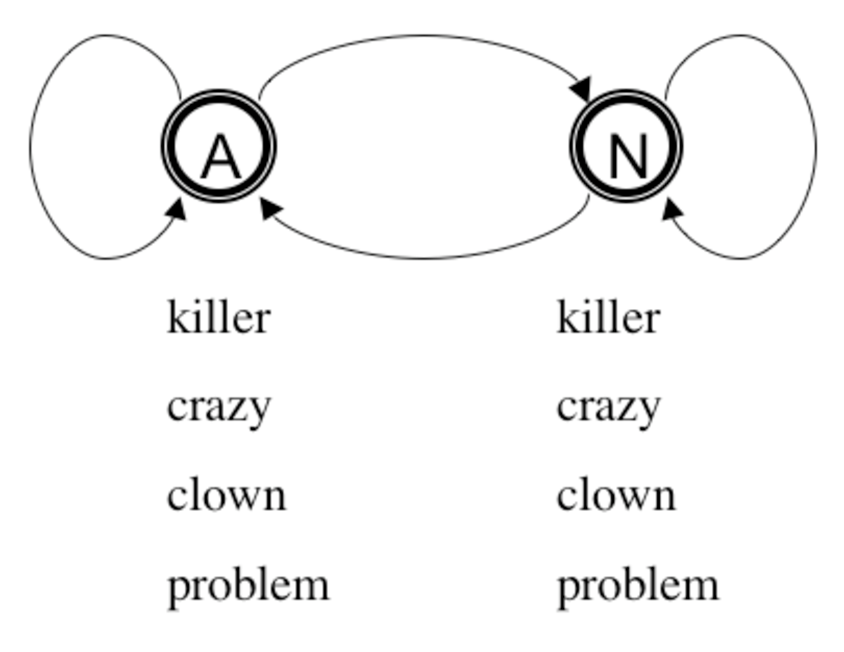
\includegraphics[scale=.4]{figures/hmmfig}
\end{center}
\end{frame}

\begin{frame}
\frametitle{Hidden Markov Model Algorithms}
\begin{itemize}
\item HMM as parser: compute the best sequence of states for a given observation sequence.
\item HMM as language model: compute probability of given observation sequence.
\item HMM as learner: given a corpus of observation sequences, learn its distribution, i.e. learn the parameters of the HMM from the corpus.
\begin{itemize}
\item Learning from a set of observations with the sequence of states provided (states are not hidden) {\color{blue} [Supervised Learning]}
\item Learning from a set of observations without any state information. {\color{blue} [Unsupervised Learning]}
\end{itemize}
\end{itemize}
\end{frame}

\section{HMM as a Language Model}

\begin{frame}
\frametitle{HMM as a Language Model}
\begin{center}
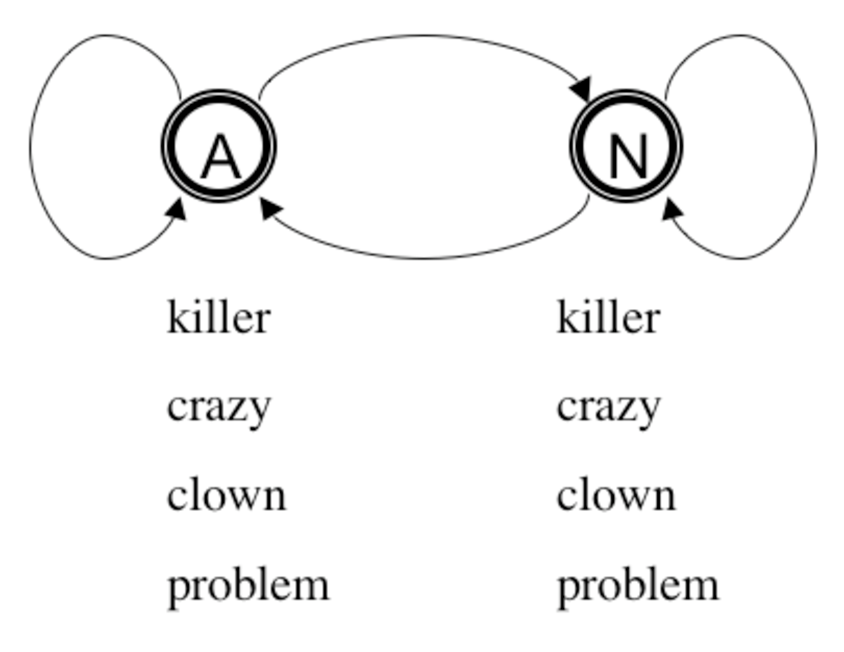
\includegraphics[scale=.3]{figures/hmmfig}
\end{center}
\begin{itemize}[<+->]
\item Find $P(\textit{killer clown}) = \sum_y P(y, \textit{killer clown})$
\item $P(\textit{killer clown}) = P(AA, \textit{killer clown}) + P(AN, \textit{killer clown}) + P(NN, \textit{killer clown}) + P(NA, \textit{killer clown})$
\end{itemize}
\end{frame}

\begin{frame}
\frametitle{HMM as a Language Model}
\begin{center}
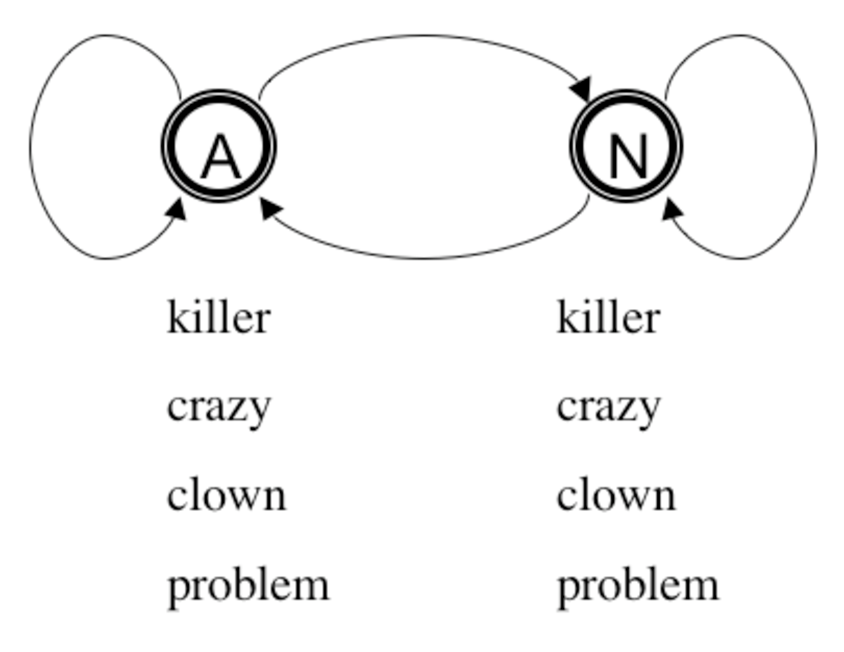
\includegraphics[scale=.3]{figures/hmmfig}
\end{center}
\begin{itemize}[<+->]
\item Consider the input {\it killer crazy clown problem}
\item So the task is to find the sum over all sequences of states:
\[ \sum_{s_1, s_2, s_3, s_4} P(\textit{killer crazy clown problem}, s_1, s_2, s_3, s_4) \]
\item A sub-problem is to find the most likely sequence of states for {\it killer crazy clown}:
\[ \sum_{s_1, s_2, s_3} P(\textit{killer crazy clown}, s_1, s_2, s_3) \]
\end{itemize}
\end{frame}

\begin{frame}
\frametitle{HMM as a Language Model}
\begin{itemize}[<+->]
\item In our example there are two possible values for $s_4$:
\begin{eqnarray*}
\lefteqn{\sum_{s_1, \ldots, s_4} P(\textit{killer crazy clown problem}, s_1, s_2, s_3, s_4) =} \\
&& {\color{blue} \sum_{s_1, s_2, s_3} P(\textit{killer crazy clown problem}, s_1, s_2, s_3, N) } + \\
&&  {\color{blue} \sum_{s_1, s_2, s_3} P(\textit{killer crazy clown problem}, s_1, s_2, s_3, A) }
\end{eqnarray*}
\item Very similar to the Viterbi algorithm. Sum instead of max, and that's the only difference!
\end{itemize}
\end{frame}

\begin{frame}
\frametitle{HMM as a Language Model}
\begin{itemize}[<+->]
\item Provide an index for each input symbol:\\
 {\it 1:killer 2:crazy 3:clown 4:problem} 
\begin{eqnarray*}
V[N, 3] &=& \sum_{s_1, s_2} P(\textit{killer crazy clown}, s_1, s_2, N) \\
V[N, 4] &=& \sum_{s_1, s_2, s_3} P(\textit{killer crazy clown problem}, s_1, s_2, s_3, N)
\end{eqnarray*}

\item Putting them together:
\begin{eqnarray*}
V[N,4] &=& {\color{blue} V[N,3] \cdot a_{N,N} \cdot b_N(\textit{problem}) } +\\
&& {\color{blue} V[A,3] \cdot a_{A,N} \cdot b_N(\textit{problem}) }
\end{eqnarray*}
\begin{eqnarray*}
V[A,4] &=& {\color{blue} V[N,3] \cdot a_{N,A} \cdot b_A(\textit{problem}) } +\\
&& {\color{blue} V[A,3] \cdot a_{A,A} \cdot b_A(\textit{problem}) }
\end{eqnarray*}
\item The best score for the input is given by:
\( V[N,4] + V[A,4] \)
\end{itemize}
\end{frame}

\begin{frame}
\frametitle{HMM as a Language Model}
\begin{itemize}[<+->]
\item For input of length $T$: $o_1, \ldots, o_T$, we want to find $P(o_1, \ldots, o_T) = \sum_{y_1, \ldots, y_T} P(y_1, \ldots, y_T, o_1, \ldots, o_T)$ 
\item Each $y_t$ in this sequence is one of the states in the HMM.
\item For each state $q$ we initialize our table: $V[q,1] = \pi_q \cdot b_q(o_1)$ 
\item Then compute recursively for $t = 1 \ldots T-1$ for each state $q$:
\[ V[q, t+1] = \sum_{q'} \left\{ V[q', t] \cdot a_{q',q} \cdot b_q(o_{t+1}) \right\} \]
\item After the loop terminates, the best score is $\sum_q V[q,T]$
\item So: Viterbi with sum instead of max gives us an algorithm for HMM as a language model.
\item This algorithm is sometimes called the \emph{forward algorithm}.
\end{itemize}
\end{frame}

\lecture{Supervised Learning for HMMs}{}

\section{Reminder: Algorithms for Hidden Markov Models}

\begin{frame}
\frametitle{Hidden Markov Model Algorithms}
\begin{itemize}
\item HMM as parser: compute the best sequence of states for a given observation sequence.
\item HMM as language model: compute probability of given observation sequence.
\item HMM as learner: given a corpus of observation sequences, learn its distribution, i.e. learn the parameters of the HMM from the corpus.
\begin{itemize}
\item Learning from a set of observations with the sequence of states provided (states are not hidden) {\color{blue} [Supervised Learning]}
\item Learning from a set of observations without any state information. {\color{blue} [Unsupervised Learning]}
\end{itemize}
\end{itemize}
\end{frame}

\section{HMM Learning: Fully Observed Case}

\begin{frame}
\frametitle{Hidden Markov Model}
\[
\textrm{Model $\theta$} = \left\{ 
\begin{array}{ll} 
\pi_i & \textrm{probability of starting at state $i$} \\ 
a_{i,j} & \textrm{probability of transition from state $i$ to state $j$} \\ 
b_i(o) & \textrm{probability of output $o$ at state $i$} \\
\end{array} 
\right. 
\]
\[
\textrm{Constraints}: \sum_i \pi_i = 1, \sum_j a_{i,j} = 1, \sum_o b_i(o) = 1
\]

\begin{center}
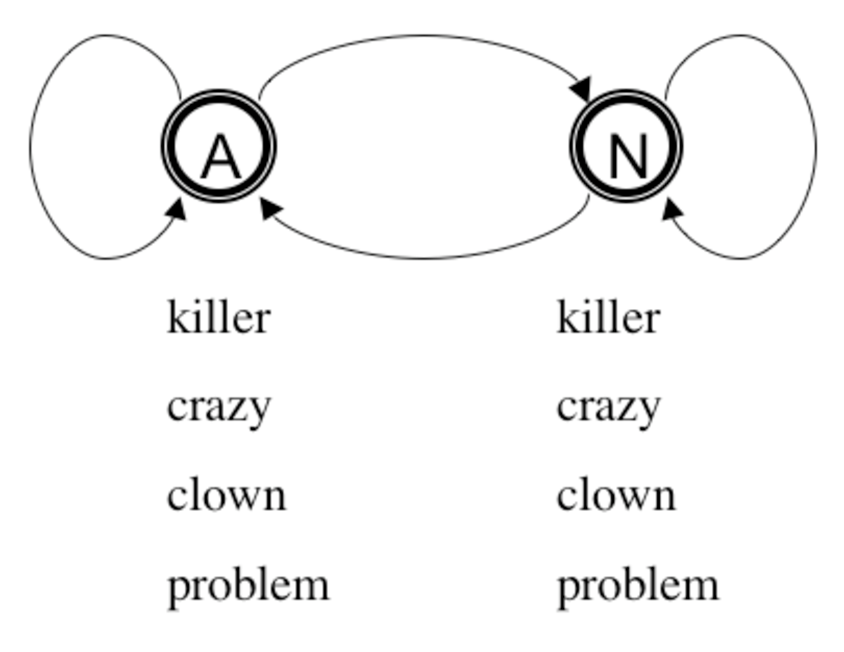
\includegraphics[scale=.4]{figures/hmmfig}
\end{center}
\end{frame}

\begin{frame}
\frametitle{HMM Learning from Labeled Data}
\begin{center}
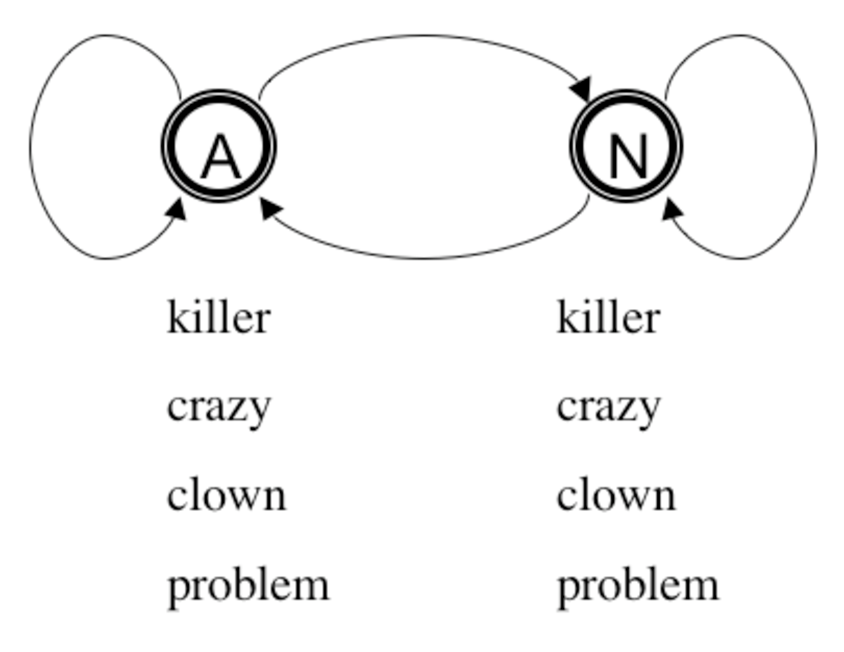
\includegraphics[scale=.4]{figures/hmmfig}
\end{center}
\begin{itemize}[<+->]
\item The task: to find the values for the parameters of the HMM:
\begin{itemize}
\item $\pi_A, \pi_N$
\item $a_{A,A}, a_{A,N}, a_{N,N}, a_{N,A}$
\item $b_A(\textit{killer}), b_A(\textit{crazy}), b_A(\textit{clown}), b_A(\textit{problem})$
\item $b_N(\textit{killer}), b_N(\textit{crazy}), b_N(\textit{clown}), b_N(\textit{problem})$
\end{itemize}
\end{itemize}
\end{frame}

\begin{frame}[fragile]
\frametitle{Learning from Fully Observed Data}
\begin{block}{Labeled Data $L$}
\begin{verbatim}
x1,y1: killer/N clown/N     (x1 = killer,clown; y1 = N,N)
x2,y2: killer/N problem/N   (x2 = killer,problem; y2 = N,N)
x3,y3: crazy/A problem/N    ...
x4,y4: crazy/A clown/N
x5,y5: problem/N crazy/A clown/N
x6,y6: clown/N crazy/A killer/N
\end{verbatim}
\end{block}
\end{frame}

\begin{frame}
\frametitle{Learning from Fully Observed Data}
\begin{itemize}[<+->]
\item Let's say we have $m$ labeled examples: $L = (x_1, y_1), \ldots, (x_m, y_m)$
\item Each $(x_\ell, y_\ell) = \{ o_1, \ldots, o_T, s_1, \ldots, s_T \}$
\item For each $(x_\ell, y_\ell)$ we can compute the probability using the HMM:
{\small\begin{itemize}[<+->]
\item $(x_1 = killer,clown; y_1 = N,N):
 {\color{blue} P(x_1, y_1) = \pi_N \cdot b_N(\textit{killer}) \cdot a_{N,N} \cdot b_N(\textit{clown})}$
\item $(x_2 = killer,problem; y_2 = N,N): 
{\color{blue} P(x_2, y_2) = \pi_N \cdot b_N(\textit{killer}) \cdot a_{N,N} \cdot b_N(\textit{problem})}$
\item $(x_3 = crazy,problem; y_3 = A,N): 
{\color{blue} P(x_3, y_3) = \pi_A \cdot b_A(\textit{crazy}) \cdot a_{A,N} \cdot b_N(\textit{problem})}$
\item $(x_4 = crazy,clown; y_4 = A,N): 
{\color{blue} P(x_4, y_4) = \pi_A \cdot b_A(\textit{crazy}) \cdot a_{A,N} \cdot b_N(\textit{clown})}$
\item $(x_5 = problem,crazy,clown; y_5 = N,A,N): 
{\color{blue} P(x_5, y_5) = \pi_N \cdot b_N(\textit{problem}) \cdot a_{N,A} \cdot b_A(\textit{crazy}) \cdot a_{A,N} \cdot b_N(\textit{clown})}$
\item $(x_6 = clown,crazy,killer; y_6 = N,A,N): 
{\color{blue} P(x_6, y_6) = \pi_N \cdot b_N(\textit{clown}) \cdot a_{N,A} \cdot b_A(\textit{crazy}) \cdot a_{A,N} \cdot b_N(\textit{killer})}$
\end{itemize}}
\item {\small\color{blue} $\prod_\ell P(x_\ell,y_\ell) \pause = {\pi_N}^{\pause 4} \pause \cdot {\pi_A}^{\pause 2} \pause \cdot {a_{N,N}}^{\pause 2} \pause \cdot {a_{N,A}}^{\pause 2} \pause \cdot {a_{A,N}}^{\pause 4} \pause \cdot {a_{A,A}}^{\pause 0} \pause \cdot {b_N(\textit{killer})}^{\pause 3} \pause \cdot {b_N(\textit{clown})}^{\pause 4} \pause \cdot {b_N(\textit{problem})}^{\pause 3} \pause \cdot {b_A(\textit{crazy})}^{\pause 4} $}
\end{itemize}
\end{frame}

\begin{frame}
\frametitle{Learning from Fully Observed Data}
\begin{itemize}[<+->]
\item We can easily collect frequency of observing a word with a state (tag)
\begin{itemize}[<+->]
\item ${\color{blue} f(i,x,y)} = $ number of times $i$ is the initial state in $(x,y)$
\item ${\color{blue} f(i,j,x,y)} = $ number of times $j$ follows $i$ in $(x,y)$
\item ${\color{blue} f(i,o,x,y)} = $ number of times $i$ is paired with observation $o$
\end{itemize}
\item Then according to our HMM the probability of $x,y$ is:
\[ P(x,y) = \prod_{i} \pi_i^{{\color{blue} f(i,x,y)}} \cdot \prod_{i,j} a_{i,j}^{{\color{blue} f(i,j,x,y)}} \cdot \prod_{i,o} b_i(o)^{{\color{blue} f(i,o,x,y)}} \]
\end{itemize}
\end{frame}

\begin{frame}
\frametitle{Learning from Fully Observed Data}
\begin{itemize}[<+->]
\item According to our HMM the probability of $x,y$ is:
\[ P(x,y) = \prod_{i} \pi_i^{f(i,x,y)} \cdot \prod_{i,j} a_{i,j}^{f(i,j,x,y)} \cdot \prod_{i,o} b_i(o)^{f(i,o,x,y)} \]
\item For the labeled data $L = (x_1, y_1), \ldots, (x_\ell, y_\ell), \ldots, (x_m, y_m)$
\begin{eqnarray*}
P(L) &=& \prod_{\ell=1}^m P(x_\ell, y_\ell) \\
&=& \prod_{\ell=1}^m \left( \prod_{i} \pi_i^{f(i,x_\ell,y_\ell)} \cdot \prod_{i,j} a_{i,j}^{f(i,j,x_\ell,y_\ell)} \cdot \prod_{i,o} b_i(o)^{f(i,o,x_\ell,y_\ell)} \right)
\end{eqnarray*}
\end{itemize}
\end{frame}

\begin{frame}
\frametitle{Learning from Fully Observed Data}
\begin{itemize}[<+->]
\item According to our HMM the probability of $x,y$ is:
\[ P(L) = \prod_{\ell=1}^m \left( \prod_{i} \pi_i^{f(i,x_\ell,y_\ell)} \cdot \prod_{i,j} a_{i,j}^{f(i,j,x_\ell,y_\ell)} \cdot \prod_{i,o} b_i(o)^{f(i,o,x_\ell,y_\ell)} \right) \]
\item The log probability of the labeled data $(x_1, y_1), \ldots, (x_m, y_m)$ according to HMM with parameters $\theta$ is:
\begin{eqnarray*}
L(\theta) & = & \sum_{\ell=1}^m \log P(x_\ell, y_\ell) \pause \\
& = & \sum_{\ell=1}^m  \sum_{i} f(i,x_\ell,y_\ell) \log \pi_i + \\
&& \sum_{i,j} f(i,j,x_\ell,y_\ell) \log a_{i,j} + \\
&& \sum_{i,o} f(i,o,x_\ell,y_\ell) \log b_i(o) 
\end{eqnarray*}
\end{itemize}
\end{frame}

\begin{frame}
\frametitle{Learning from Fully Observed Data}
{\small\begin{eqnarray*}
\lefteqn{L(\theta) = \sum_{\ell=1}^m  } \\
&& \sum_{i} f(i,x_\ell,y_\ell) \log \pi_i + \sum_{i,j} f(i,j,x_\ell,y_\ell) \log a_{i,j} + \sum_{i,o} f(i,o,x_\ell,y_\ell) \log b_i(o) \end{eqnarray*}}
\begin{itemize}[<+->]
\item $\theta = \left( \pi, a, b \right)$
\item $L(\theta)$ is the log probability of the labeled data $(x_1, y_1), \ldots, (x_m, y_m)$ 
\item We want to find a $\theta$ that will give us the maximum value of $L(\theta)$
\item Find the $\theta$ such that $\frac{d L(\theta)}{d \theta} = 0$ 
\end{itemize}
\end{frame}

\begin{frame}
\frametitle{Learning from Fully Observed Data}
{\small\begin{eqnarray*}
\lefteqn{L(\theta) = \sum_{\ell=1}^m  } \\
&& \sum_i f(i,x_\ell,y_\ell) \log \pi_i + \sum_{i,j} f(i,j,x_\ell,y_\ell) \log a_{i,j} + \sum_{i,o} f(i,o,x_\ell,y_\ell) \log b_i(o) \end{eqnarray*}}
\begin{itemize}[<+->]
\item The values of $\pi_i, a_{i,j}, b_i(o)$ that maximize $L(\theta)$ are:
\begin{eqnarray*}
\pi_i & = & \frac{\sum_\ell f(i,x_\ell,y_\ell)}{\sum_\ell \sum_k f(k,x_\ell,y_\ell)} \\
a_{i,j} & = & \frac{\sum_\ell f(i,j,x_\ell,y_\ell)}{\sum_\ell \sum_k f(i,k,x_\ell,y_\ell)} \\
b_i(o) & = & \frac{\sum_\ell f(i,o,x_\ell,y_\ell)}{\sum_\ell \sum_{o' \in V} f(i,o',x_\ell,y_\ell)} 
\end{eqnarray*}
\end{itemize}
\end{frame}


\begin{frame}[fragile]
\frametitle{Learning from Fully Observed Data}
\begin{block}{Labeled Data:}
\begin{verbatim}
x1,y1: killer/N clown/N       
x2,y2: killer/N problem/N     
x3,y3: crazy/A problem/N
x4,y4: crazy/A clown/N
x5,y5: problem/N crazy/A clown/N
x6,y6: clown/N crazy/A killer/N
\end{verbatim}
\end{block}
\end{frame}

\begin{frame}
\frametitle{Learning from Fully Observed Data}
\begin{itemize}[<+->]
\item The values of $\pi_i$ that maximize $L(\theta)$ are:
\begin{eqnarray*}
\pi_i & = & \frac{\sum_\ell f(i,x_\ell,y_\ell)}{\sum_\ell \sum_k f(k,x_\ell,y_\ell)} 
\end{eqnarray*}
\item $\pi_N = \frac{2}{3}$ and $\pi_A = \frac{1}{3}$ because:
\begin{eqnarray*}
\sum_\ell f(N, x_\ell, y_\ell) & = & 4 \\
\sum_\ell f(A, x_\ell, y_\ell) & = & 2 
\end{eqnarray*}
\end{itemize}
\end{frame}

\begin{frame}
\frametitle{Learning from Fully Observed Data}
\begin{itemize}[<+->]
\item The values of $a_{i,j}$ that maximize $L(\theta)$ are:
\begin{eqnarray*}
a_{i,j} & = & \frac{\sum_\ell f(i,j,x_\ell,y_\ell)}{\sum_\ell \sum_k f(i,k,x_\ell,y_\ell)} 
\end{eqnarray*}
\item $a_{N,N} = \frac{1}{2}$ ; $a_{N,A} = \frac{1}{2}$ ; $a_{A,N} = 1$ and $a_{A,A} = 0$ because:
\end{itemize}

\begin{columns}[c]
\column{2in}
\begin{eqnarray*}
\sum_\ell f(N, N, x_\ell, y_\ell) & = & 2 \\
\sum_\ell f(N, A, x_\ell, y_\ell) & = & 2 
\end{eqnarray*}

\column{1.5in}
\begin{eqnarray*}
\sum_\ell f(A, N, x_\ell, y_\ell) & = & 4 \\ 
\sum_\ell f(A, A, x_\ell, y_\ell) & = & 0 
\end{eqnarray*}
\end{columns}
\end{frame}

\begin{frame}
\frametitle{Learning from Fully Observed Data}
\begin{itemize}[<+->]
\item The values of $b_{i}(o)$ that maximize $L(\theta)$ are:
\begin{eqnarray*}
b_i(o) & = & \frac{\sum_\ell f(i,o,x_\ell,y_\ell)}{\sum_\ell \sum_{o' \in V} f(i,o',x_\ell,y_\ell)} 
\end{eqnarray*}
\item $b_{N}(\textit{killer}) = \frac{3}{10}$ ;  $b_{N}(\textit{clown}) = \frac{4}{10}$ ; $b_{N}(\textit{problem}) = \frac{3}{10}$ and $b_{A}(\textit{crazy}) = 1$ because:
\end{itemize}

\begin{columns}[c]

\column{2in}
{\small\begin{eqnarray*}
\sum_\ell f(N, \textit{killer}, x_\ell, y_\ell) & = & 3 \\
\sum_\ell f(N, \textit{clown}, x_\ell, y_\ell) & = & 4 \\ 
\sum_\ell f(N, \textit{crazy}, x_\ell, y_\ell) & = & 0 \\ 
\sum_\ell f(N, \textit{problem}, x_\ell, y_\ell) & = & 3 \\ 
\end{eqnarray*}}

\column{1.5in}
{\small\begin{eqnarray*}
\sum_\ell f(A, \textit{killer}, x_\ell, y_\ell) & = & 0 \\
\sum_\ell f(A, \textit{clown}, x_\ell, y_\ell) & = & 0 \\ 
\sum_\ell f(A, \textit{crazy}, x_\ell, y_\ell) & = & 4 \\ 
\sum_\ell f(A, \textit{problem}, x_\ell, y_\ell) & = & 0 \\ 
\end{eqnarray*}}

\end{columns}
\end{frame}

\begin{frame}[fragile]
\frametitle{Learning from Fully Observed Data}
\begin{verbatim}
x1,y1: killer/N clown/N       
x2,y2: killer/N problem/N     
x3,y3: crazy/A problem/N
x4,y4: crazy/A clown/N
x5,y5: problem/N crazy/A clown/N
x6,y6: clown/N crazy/A killer/N
\end{verbatim}

\begin{columns}[c]
\column{1in}
\[ \pi = \begin{array}{|l|l|}
\hline
A & 0.25 \\ \hline
N & 0.75 \\ \hline
\end{array}
\]

\column{1in}
\[ a = \begin{array}{|l|l|l|}
\hline
a_{i,j} & A & N \\ \hline
A & 0.0 & 1.0 \\ \hline
N & 0.5 & 0.5 \\ \hline
\end{array}
\]
\end{columns}

\[ b = \begin{array}{|l|l|l|l|l|}
\hline
b_i(o) & clown & killer & problem & crazy \\ \hline
A & 0 & 0 & 0 & 1 \\ \hline
N & 0.4 & 0.3 & 0.3 & 0 \\ \hline
\end{array}
\]

\end{frame}

\lecture{Lagrange Multipliers}{}

\section{HMM Learning: Fully Observed Case}

\begin{frame}
\frametitle{Hidden Markov Model}
\[
\textrm{Model $\theta$} = \left\{ 
\begin{array}{ll} 
\pi_i & \textrm{$p(i)$: starting at state $i$} \\ 
a_{i,j} & \textrm{$p(j \mid i)$: transition to state $i$ from state $j$} \\ 
b_i(o) & \textrm{$p( o \mid i)$: output $o$ at state $i$}
\end{array} 
\right.\]

\begin{center}
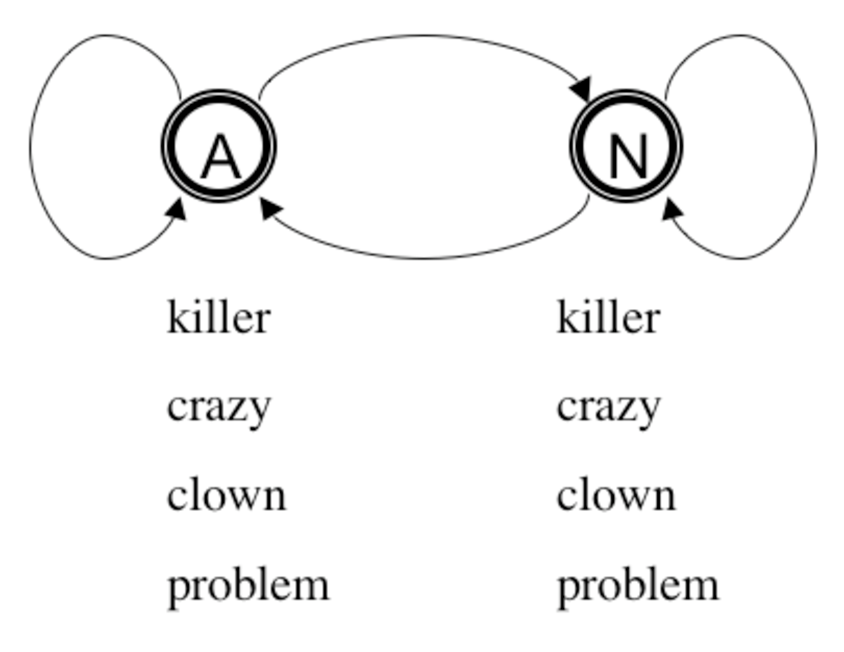
\includegraphics[scale=.4]{figures/hmmfig}
\end{center}
\end{frame}

\begin{frame}
\frametitle{Learning from Fully Observed Data}
{\small\begin{eqnarray*}
\lefteqn{L(\theta) = \sum_{\ell=1}^m  } \\
&& \sum_{i} f(i,x_\ell,y_\ell) \log \pi_i + \sum_{i,j} f(i,j,x_\ell,y_\ell) \log a_{i,j} + \sum_{i,o} f(i,o,x_\ell,y_\ell) \log b_i(o) \end{eqnarray*}}
\begin{itemize}[<+->]
\item $\theta = \left( \pi, a, b \right)$
\item $L(\theta)$ is the log probability of the labeled data $(x_1, y_1), \ldots, (x_m, y_m)$ 
\item We want to find a $\theta$ that will give us the maximum value of $L(\theta)$
\item Find the $\theta$ such that $\frac{d L(\theta)}{d \theta} = 0$ 
\end{itemize}
\end{frame}

\begin{frame}
\frametitle{Learning from Fully Observed Data}
{\small\begin{eqnarray*}
\lefteqn{L(\theta) = \sum_{\ell=1}^m  } \\
&& \sum_i f(i,x_\ell,y_\ell) \log \pi_i + \sum_{i,j} f(i,j,x_\ell,y_\ell) \log a_{i,j} + \sum_{i,o} f(i,o,x_\ell,y_\ell) \log b_i(o) \end{eqnarray*}}
\begin{itemize}[<+->]
\item Find the $\theta$ such that $\frac{d L(\theta)}{d \theta} = 0$ and $\theta = \left( \pi, a, b \right)$
\item Split up $L(\theta)$ into $L(\pi), L(a), L(b)$
\item Let $\nabla L = \forall i,j,o: \frac{\partial L(\pi)}{\partial \pi_i} \, , \, \frac{\partial L(a)}{\partial a_{i,j}} \, , \, \frac{\partial L(b)}{\partial b_i(o)}$
\item We must also obey constraints: $\sum_k \pi_k = 1, \sum_k a_{i,k} = 1, \sum_o b_i(o) = 1$
\end{itemize}
\end{frame}

\begin{frame}
\frametitle{Learning from Fully Observed Data}
{\small\begin{eqnarray*} L(\pi) = \sum_{\ell=1}^m \sum_i f(i,x_\ell,y_\ell) \log \pi_i \end{eqnarray*}}
\begin{itemize}[<+->]
\item Let us focus on $\nabla L(\pi)$ (the other two: $a$ and $b$ are similar)
\item For the constraint $\sum_k \pi_k = 1$ we introduce a new variable into our search for a maximum:
\[ L(\pi, \lambda) = L(\pi) + \lambda ( 1 - \sum_k \pi_k ) \]
\item $\lambda$ is called the Lagrange multiplier
\item $\lambda$ penalizes any solution that does not obey the constraint
\item The constraint ensures that $\pi$ is a probability distribution
\end{itemize}
\end{frame}

\begin{frame}
\frametitle{Learning from Fully Observed Data}
{\small\begin{eqnarray*} \frac{\partial L(\pi)}{\partial \pi_i} = \frac{\partial }{\partial \pi_i} \underbrace{\sum_{\ell=1}^m f(i,x_\ell,y_\ell) \log \pi_i}_{\textrm{the only part with variable $\pi_i$}} + \underbrace{\sum_{\ell=1}^m \sum_{j : j \neq i}  f(j,x_\ell,y_\ell) \log \pi_j}_{\textrm{no $\pi_i$ so derivative is $0$}} \end{eqnarray*}}
\begin{itemize}[<+->]
\item We want a value of $\pi_i$ such that $\frac{\partial L(\pi, \lambda)}{\partial \pi_i} = 0$ \pause
\begin{eqnarray*}
\frac{\partial }{\partial \pi_i} \sum_{\ell=1}^m \left( f(i,x_\ell,y_\ell) \log \pi_i + \lambda ( 1 - \sum_k \pi_k ) \right) = 0 \pause \\
\frac{\partial }{\partial \pi_i} \sum_{\ell=1}^m \left( \underbrace{\textcolor{blue}{f(i,x_\ell,y_\ell) \log \pi_i}}_{\textcolor{red}{\frac{\partial }{\partial \pi_i}=\frac{f(i,x_\ell,y_\ell)}{\pi_i}}} + \lambda - \underbrace{\textcolor{blue}{\lambda \pi_i}}_{\textcolor{red}{\frac{\partial }{\partial \pi_i}=\lambda}} - \lambda \sum_{j : j \neq i} \pi_j ) \right) = 0 
\end{eqnarray*}
\end{itemize}
\end{frame}

\begin{frame}
\frametitle{Learning from Fully Observed Data}
{\small\begin{eqnarray*} \frac{\partial L(\pi)}{\partial \pi_i} = \frac{\partial }{\partial \pi_i} \underbrace{\sum_{\ell=1}^m f(i,x_\ell,y_\ell) \log \pi_i}_{\textrm{the only part with variable $\pi_i$}} + \underbrace{\sum_{\ell=1}^m \sum_{j : j \neq i}  f(j,x_\ell,y_\ell) \log \pi_j}_{\textrm{no $\pi_i$ so derivative is $0$}} \end{eqnarray*}}
\begin{itemize}[<+->]
\item We can obtain a value of $\pi_i$ wrt $\lambda$: \pause
\begin{eqnarray}
\frac{\partial L(\pi, \lambda)}{\partial \pi_i} = \underbrace{\textcolor{red}{\sum_{\ell=1}^m \frac{f(i,x_\ell,y_\ell)}{\pi_i} - \lambda}}_{\textrm{\textcolor{blue}{see previous slide}}} = 0 \nonumber \pause \\
\pi_i = \frac{\sum_{\ell=1}^m f(i, x_\ell, y_\ell)}{\lambda} \label{eqn:pidef}
\end{eqnarray}
\item Combine $\pi_i$s from Eqn~(\ref{eqn:pidef}) with constraint $\sum_k \pi_k = 1$
\begin{eqnarray*}
\lambda = \sum_k \sum_{\ell=1}^m f(k, x_\ell, y_\ell)
\end{eqnarray*}
\end{itemize}
\end{frame}

\begin{frame}
\frametitle{Learning from Fully Observed Data}
{\small\begin{eqnarray*} \frac{\partial L(\pi)}{\partial \pi_i} = \frac{\partial }{\partial \pi_i} \underbrace{\sum_{\ell=1}^m f(i,x_\ell,y_\ell) \log \pi_i}_{\textrm{the only part with variable $\pi_i$}} + \underbrace{\sum_{\ell=1}^m \sum_{j : j \neq i}  f(j,x_\ell,y_\ell) \log \pi_j}_{\textrm{no $\pi_i$ so derivative is $0$}} \end{eqnarray*}}
\begin{itemize}[<+->]
\item The value of $\pi_i$ for which $\frac{\partial L(\pi, \lambda)}{\partial \pi_i} = 0$ is Eqn~(\ref{eqn:pidef2}) which can be combined with the value of $\lambda$ from Eqn~(\ref{eqn:lambdadef}).
\begin{eqnarray}
\pi_i = \frac{\sum_{\ell=1}^m f(i, x_\ell, y_\ell)}{\textcolor{red}{\lambda}} \label{eqn:pidef2} \\
\textcolor{red}{\lambda = \sum_k \sum_{\ell=1}^m f(k, x_\ell, y_\ell)} \label{eqn:lambdadef} \\
\textcolor{blue}{\pi_i = \frac{\sum_{\ell=1}^m f(i, x_\ell, y_\ell)}{\sum_k \sum_{\ell=1}^m f(k, x_\ell, y_\ell)}}  \nonumber
\end{eqnarray}
\end{itemize}
\end{frame}

\begin{frame}
\frametitle{Learning from Fully Observed Data}
{\small\begin{eqnarray*}
\lefteqn{L(\theta) = \sum_{\ell=1}^m  } \\
&& \sum_i f(i,x_\ell,y_\ell) \log \pi_i + \sum_{i,j} f(i,j,x_\ell,y_\ell) \log a_{i,j} + \sum_{i,o} f(i,o,x_\ell,y_\ell) \log b_i(o) \end{eqnarray*}}
\begin{itemize}[<+->]
\item The values of $\pi_i, a_{i,j}, b_i(o)$ that maximize $L(\theta)$ are:
\begin{eqnarray*}
\pi_i & = & \frac{\sum_\ell f(i,x_\ell,y_\ell)}{\sum_\ell \sum_k f(k,x_\ell,y_\ell)} \\
a_{i,j} & = & \frac{\sum_\ell f(i,j,x_\ell,y_\ell)}{\sum_\ell \sum_k f(i,k,x_\ell,y_\ell)} \\
b_i(o) & = & \frac{\sum_\ell f(i,o,x_\ell,y_\ell)}{\sum_\ell \sum_{o' \in V} f(i,o',x_\ell,y_\ell)} 
\end{eqnarray*}
\end{itemize}
\end{frame}

\lecture{Unsupervised Learning for HMMs}

\section{Reminder: Algorithms for Hidden Markov Models}

\begin{frame}
\frametitle{Hidden Markov Model}
\[
\textrm{Model $\theta$} = \left\{ 
\begin{array}{ll} 
\pi_i & \textrm{$p(i)$: starting at state $i$} \\ 
a_{i,j} & \textrm{$p(j \mid i)$: transition to state $i$ from state $j$} \\ 
b_i(o) & \textrm{$p( o \mid i)$: output $o$ at state $i$}
\end{array} 
\right.\]

\begin{center}
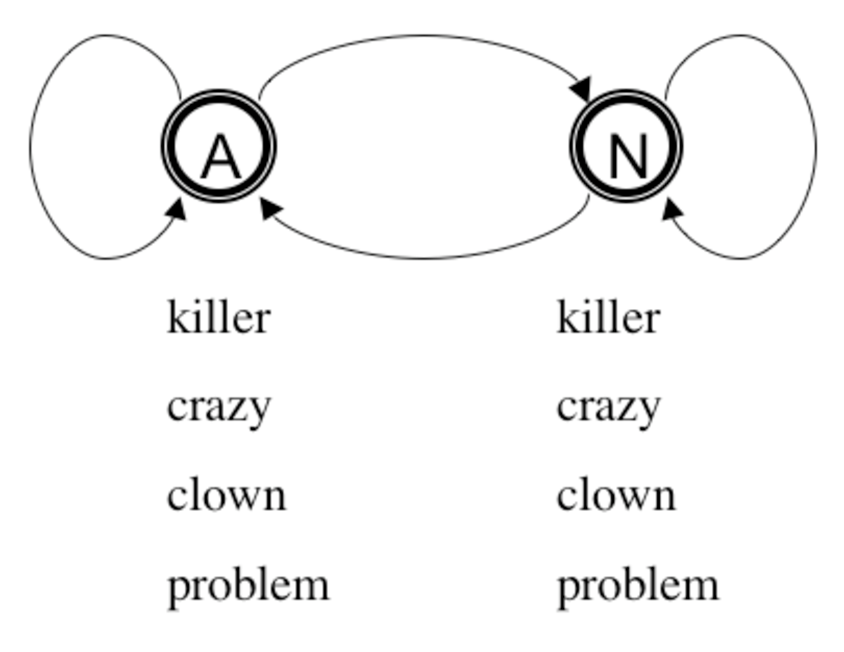
\includegraphics[scale=.4]{figures/hmmfig}
\end{center}
\end{frame}

\begin{frame}
\frametitle{Hidden Markov Model Algorithms}
\begin{itemize}
\item HMM as parser: compute the best sequence of states for a given observation sequence.
\item HMM as language model: compute probability of given observation sequence.
\item HMM as learner: given a corpus of observation sequences, learn its distribution, i.e. learn the parameters of the HMM from the corpus.
\begin{itemize}
\item Learning from a set of observations with the sequence of states provided (states are not hidden) {\color{blue} [Supervised Learning]}
\item Learning from a set of observations without any state information. {\color{blue} [Unsupervised Learning]}
\end{itemize}
\end{itemize}
\end{frame}

\section{Learning from Unlabeled Data}

\begin{frame}[fragile]
\frametitle{Learning from Unlabeled Data}
\begin{block}{Unlabeled Data $U = x_1, \ldots, x_m$:}
\begin{verbatim}
x1: killer clown
x2: killer problem
x3: crazy problem
x4: crazy clown
\end{verbatim}
\end{block}

\begin{itemize}[<+->]
\item {\tt y1, y2, y3, y4} are unknown.
\item But we can enumerate all possible values for {\tt y1, y2, y3, y4}
\item For example, for {\tt x1: killer clown}
{\small\begin{tabular}{ll}
\pause
{\tt x1,y1,1: killer/A clown/A} & $p_1 = \pi_A \cdot b_A(\textit{killer}) \cdot a_{A,A} \cdot b_A(\textit{clown})$ \\
\pause
{\tt x1,y1,2: killer/A clown/N} & $p_2 = \pi_A \cdot b_A(\textit{killer}) \cdot a_{A,N} \cdot b_N(\textit{clown})$\\
\pause
{\tt x1,y1,3: killer/N clown/N} & $p_3 = \pi_N \cdot b_N(\textit{killer}) \cdot a_{N,N} \cdot b_N(\textit{clown})$\\
\pause
{\tt x1,y1,4: killer/N clown/A} & $p_4 = \pi_N \cdot b_N(\textit{killer}) \cdot a_{N,A} \cdot b_A(\textit{clown})$
\end{tabular}}
\end{itemize}
\end{frame}


\begin{frame}
\frametitle{Learning from Unlabeled Data}
\begin{itemize}[<+->]
\item Assume some values for $\theta = \pi, a, b$
\item We can compute $P(y \mid x_\ell, \theta)$ for any $y$ for a given $x_\ell$
\[ P(y \mid x_\ell, \theta) = \frac{ P(x, y \mid \theta) }{ \sum_{y'} P(x, y' \mid \theta) } \]
\item For example, we can compute $P( \texttt{NN} \mid \texttt{killer clown}, \theta)$ as follows:
\[ \frac{ \pi_N \cdot b_N(\textit{killer}) \cdot a_{N,N} \cdot b_N(\textit{clown}) }
{ \sum_{i,j} \pi_i \cdot b_i(\textit{killer}) \cdot a_{i,j} \cdot b_j(\textit{clown}) } \]
\item $P(y \mid x_\ell, \theta)$ is called the \emph{posterior probability}
\end{itemize}
\end{frame}

\begin{frame}
\frametitle{Learning from Unlabeled Data}
\begin{itemize}[<+->]
\item Compute the posterior for all possible outputs for each example in training:
\item For {\tt x1: killer clown} \pause
{\small\begin{tabular}{ll}
{\tt x1,y1,1: killer/A clown/A} & $P(\texttt{AA} \mid \texttt{killer clown}, \theta)$ \pause \\
{\tt x1,y1,2: killer/A clown/N} & $P(\texttt{AN} \mid \texttt{killer clown}, \theta)$ \pause \\
{\tt x1,y1,3: killer/N clown/N} & $P(\texttt{NN} \mid \texttt{killer clown}, \theta)$ \pause \\
{\tt x1,y1,4: killer/N clown/A} & $P(\texttt{NA} \mid \texttt{killer clown}, \theta)$
\end{tabular}}
\item For {\tt x2: killer problem}
{\small\begin{tabular}{ll}
{\tt x2,y2,1: killer/A problem/A} & $P(\texttt{AA} \mid \texttt{killer problem}, \theta)$ \\
{\tt x2,y2,2: killer/A problem/N} & $P(\texttt{AN} \mid \texttt{killer problem}, \theta)$\\
{\tt x2,y2,3: killer/N problem/N} & $P(\texttt{NN} \mid \texttt{killer problem}, \theta)$\\
{\tt x2,y2,4: killer/N problem/A} & $P(\texttt{NA} \mid \texttt{killer problem}, \theta)$
\end{tabular}}
\item Similarly for {\tt x3: crazy problem} 
\item And {\tt x4: crazy clown}
\end{itemize}
\end{frame}


\begin{frame}
\frametitle{Learning from Unlabeled Data}
\begin{itemize}[<+->]
\item For unlabeled data, the log probability of the data given $\theta$ is:
\begin{eqnarray*}
 L(\theta) &=& \sum_{\ell=1}^m \log \sum_y P(x_\ell,y \mid \theta) \\
 &=& \sum_{\ell=1}^m \log \sum_y P(y \mid x_\ell, \theta) \cdot P(x_\ell \mid \theta)
 \end{eqnarray*}
\item Unlike the fully observed case there is no simple solution to finding $\theta$ to maximize $L(\theta)$
\item We instead initialize $\theta$ to some values, and then iteratively find better values of $\theta$: $\theta^0, \theta^1, \ldots$ using the following formula:
\begin{eqnarray*}
\theta^t &=& \arg\max_\theta Q(\theta, \theta^{t-1})\\
&=& \sum_{\ell=1}^m \sum_y P(y \mid x_\ell, \theta^{t-1}) \cdot \log P(x_\ell, y \mid \theta) 
\end{eqnarray*}
\end{itemize}
\end{frame}

\begin{frame}
\frametitle{Learning from Unlabeled Data}
\begin{eqnarray*}
\theta^t &=& \arg\max_\theta Q(\theta, \theta^{t-1})\\
Q(\theta, \theta^{t-1}) &=& \sum_{\ell=1}^m \sum_y P(y \mid x_\ell, \theta^{t-1}) \cdot {\color{blue} \log P(x_\ell, y \mid \theta)} \\
&=& \sum_{\ell=1}^m \sum_y P(y \mid x_\ell, \theta^{t-1}) \cdot \\
&& \left( {\color{blue}  \sum_i f(i, x_\ell, y) \cdot \log \pi_i } \right. \\
&& {\color{blue} + \sum_{i,j} f(i,j,x_\ell,y) \cdot \log a_{i,j} } \\
&& \left. {\color{blue} + \sum_{i,o} f(i,o,x_\ell,y) \cdot \log b_i(o) } \right)
\end{eqnarray*}
\end{frame}

\begin{frame}
\frametitle{Learning from Unlabeled Data}
\begin{eqnarray*}
g(i,x_\ell) &=& \sum_y P(y \mid x_\ell, \theta^{t-1}) \cdot f(i, x_\ell, y) \\
g(i,j,x_\ell) &=& \sum_y P(y \mid x_\ell, \theta^{t-1}) \cdot f(i, j, x_\ell, y) \\
g(i,o,x_\ell) &=& \sum_y P(y \mid x_\ell, \theta^{t-1}) \cdot f(i, o, x_\ell, y)
\end{eqnarray*}
\begin{eqnarray*}
\theta^t & = & \arg\max_{\pi,a,b} \sum_{\ell=1}^m \sum_i g(i,x_\ell) \cdot \log \pi_i \\
&& + \sum_{i,j} g(i,j,x_\ell) \cdot \log a_{i,j} \\
&& + \sum_{i,o} g(i,o,x_\ell) \cdot \log b_j(o)
\end{eqnarray*}
\end{frame}

\begin{frame}
\frametitle{Learning from Unlabeled Data}
{\small\begin{eqnarray*}
\lefteqn{Q(\theta,\theta^{t-1}) = \sum_{\ell=1}^m  } \\
&& \sum_i g(i,x_\ell) \log \pi_i + \sum_{i,j} g(i,j,x_\ell) \log a_{i,j} + \sum_{i,o} g(i,o,x_\ell) \log b_i(o) \end{eqnarray*}}
\begin{itemize}[<+->]
\item The values of $\pi_i, a_{i,j}, b_i(o)$ that maximize $L(\theta)$ are:
\begin{eqnarray*}
\pi_i & = & \frac{\sum_\ell g(i,x_\ell)}{\sum_\ell \sum_k g(k,x_\ell)} \\
a_{i,j} & = & \frac{\sum_\ell g(i,j,x_\ell)}{\sum_\ell \sum_k g(i,k,x_\ell)} \\
b_i(o) & = & \frac{\sum_\ell g(i,o,x_\ell)}{\sum_\ell \sum_{o' \in V} g(i,o',x_\ell)} 
\end{eqnarray*}
\end{itemize}
\end{frame}

\begin{frame}
\frametitle{EM Algorithm for Learning HMMs}
\begin{itemize}[<+->]
\item Initialize $\theta^0$ at random. Let $t=0$.
\item The EM Algorithm:
\begin{itemize}[<+->]
\item E-step: compute expected values of $y$, $P(y \mid x, \theta)$ and calculate $g(i,x), g(i,j,x), g(i,o,x)$
\item M-step: compute $\theta^{t} = \arg\max_\theta Q(\theta, \theta^{t-1})$
\item Stop if $L(\theta^t)$ did not change much since last iteration. Else continue.
\end{itemize}
\item The above algorithm is guaranteed to improve likelihood of the unlabeled data.
\item In other words, $L(\theta^t) \geq L(\theta^{t-1})$
\item \emph{But} it all depends on $\theta^0$!
\end{itemize}
\end{frame}



\section*{Acknowledgements}

\begin{frame}
\centering
\begin{alertblock}{Acknowledgements}
Many slides borrowed or inspired from lecture notes by Michael Collins, Chris Dyer, Kevin Knight, Philipp Koehn, Adam Lopez, and Luke Zettlemoyer from their NLP course materials. 

\bigskip

All mistakes are my own.
\end{alertblock}
\end{frame}



\end{document}
